\documentclass[12pt]{report}
  \title{\LARGE Distributed simulation of spiking neural networks using Message Passing Interface \\ \vspace{7mm} \large Final Year Project}
  \author{ \emph{Author:} \\ Iskander Orazbekov \vspace{5 mm} \\ \emph{Supervisor:} \\ Dr Timothy Todman \vspace{5 mm} \\ \emph{Second Marker:} \\ Professor Murray Shanahan \vspace{56 mm} \\ Imperial College London}
  \date{\today}
\usepackage{a4}
\usepackage{listings}
\lstset{
	language=C++,
	frame=single,
	numbers=left,
	breaklines=true,
	breakautoindent=true,
	xleftmargin={\ifodd\value{page}1em\else-\marginparwidth\fi},
	xrightmargin={\ifodd\value{page}-\marginparwidth\else1em\fi},
	basicstyle=\ttfamily\footnotesize\bfseries,
	frame=tb
}
\usepackage{graphicx}
\usepackage{url}
\usepackage[english]{babel}
\usepackage{wrapfig}
\usepackage[toc,page]{appendix}
\setlength{\parskip}{0.3cm}
\setlength{\parindent}{0cm}

\begin{document}

\maketitle

\begin{abstract}

Motivation behind the development of spiking neural networks arised from the growing interest in the area of neural 
computation and studies of brain activity in the recent years. The reason lies in the fact that SNNs incorporate time
into neuron firing computation and signify the role of interconnectedness between neurons, therefore bringing the simulation 
level closer to reality.

However, as a result of such improvement, spiking neural networks are computationally expensive to simulate, therefore, a solution 
using parallel computation was needed. NeMo, a Spiking Neural Network simulator developed at Imperial College, solves this problem 
by making use of CUDA-interfaced GPUs with high level of parallelism.

The aim of this project is to implement the Message Passing Interface for NeMo, and by doing this, improve inter-neural communication, 
to allow for better performance of parallel computations. This, in turn, will allow for bigger number of neurons within the network 
and greater level of realism brought by the simulation.

\end{abstract}

\clearpage

\chapter*{Acknowledgements}
\thispagestyle{empty}

I would like to thank...

\clearpage

\tableofcontents

\renewcommand{\chaptername}{}

\chapter{Introduction}

Studies in the area of neuroscience have always pushed boundaries of the development of simulation tools, requiring more computational power 
for realistical models. In order to achieve a high level of realism, large-scale networks are needed, that consist of more than \begin{math}10^8\end{math} neurons 
and \begin{math}10^{12}\end{math} synapses - and manipulating that data alone comprises a challenging task.

Consequently, parallel computations are used, in order to minimize the workload given to a particular machine and to ensure that throughout
this execution all of the clusters are communicating between each other. Once implemented, this system will allow a great amount of scalability
to be put to use, enhancing the quality of simulations.

Therefore, \emph{Message Passing Interface} (MPI) improvement in the current NeMo system will allow for faster rate of computations by making use 
of parallelism. With the use of MPI, it will be possible to make full use of cluster-based implementation that will deal with the scalability by 
distributing the workload across several machines. This means that a simulation would be able to host more neurons, therefore creating a more 
realistical model of brain activity and making it more useful for the research purposes.

However, bigger number of neurons results in need for more efficient memory management, as more data would have to be stored for effective 
communication. At the same time, a mapping specific to the topology and interconnectedness of a particular network should be derived to increase
the efficiency of transmissions.

All in all, the successful implementation of the MPI communications protocol will achieve not only a greater scope of usage of NeMo simulator within
neural computing research, but also provide a good basis for future implementations and enhancements of the simulator.


\chapter{Background}

This chapter will outline the information needed for better understanding of the idea of the project and its underlying processes.

\section{Spiking Neural Networks}

An \emph{artificial neural network}(ANN) is defined as a computational model inspired by the structure and functional aspects of biological neural networks.\cite{ActFunc}
It is an adaptive system that consists of \textbf{neurons}, its basic computational units, that are connected with each other via \textbf{synapses}.
Modern neural networks are mostly used as non-linear statistical data modeling tools to find patterns between inputs and outputs.\cite{Bar-Yam2003}

\emph{Spiking neural network}(SNN) - is a third generation neural network that comprises within itself not only concepts of neuronal and synaptic states, but 
also time.\cite{Maass1997} As a result of putting emphasis on time as an acting property, a much higher level of realism is achieved in simulations,
making SNNs particularly useful for research in such areas as brain activity or neural computation.

\subsection{Artificial and Spiking Neurons}

In order to distinguish between different generations of neural networks, one would need to take into account type of neurons, as they define the type of network.

\begin{figure}[h]
\begin{center}
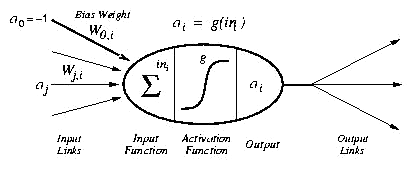
\includegraphics[scale = 0.6]{images/neuron_model.png}
\end{center}
\caption{A graphical model of a simple artificial neuron\cite{Philosophy}}
\end{figure}

Typical neural networks consist of a number of computational units, \emph{artificial neurons}. An \emph{artificial neuron} is a model of a mathematical 
function or an abstraction of biological neurons\cite{Harmon1959}, that given several inputs, derives a value based on the sum of this collection of inputs 
and built-in function, and returns this value as an output, essentially acting as an axon of a real neuron. Artificial neurons differ depending on their 
specific model, such as McCulloch-Pitts or linear-threshold function. These models define a set of properties that a particular neuron possesses, such as 
transfer (or activation) function.

\begin{figure}[h]
\begin{center}
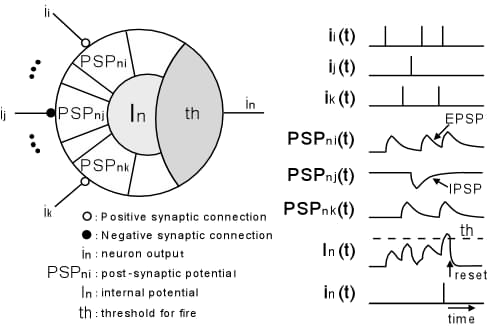
\includegraphics[scale = 0.8]{images/spiking-model.png}
\end{center}
\caption{A graphical model of a spiking neuron\cite{HidekiTanaka2009}}
\end{figure}

However, spiking neural networks are quite different in nature and, specifically, in structure of their computational units from artificial neural networks. SNNs consist of \textbf{spiking neurons} 
that aim to model the activity of real biological neurons, that is to make an abstraction which is as close as possible to the original. A \emph{spiking neuron} instead of
having set time period of emission, fires a \textbf{spike} - a very short signal that remains at its peak value for about a millisecond. Firing in spiking neurons is caused
by changes in membrane potential as well as resulting from time-based activation function. The signal is transferred to other neurons, in turn, increasing or decreasing their
membrane potential. However, since signals do not vary in value, the information is transferred via a collection of spikes, called a \emph{spike train}. Through the spike train
it is relatively easy to obtain the timing and number of spikes, therefore, these two variables hold the actual data.\cite{WulframGerstner2002} By possessing these qualities, networks 
built from spiking neurons obtain a significantly larger computational power than that of same-sized artificial neural network.\cite{Maass2003}

\subsubsection{Activation Function}

An activation function is usually an abstraction that represents the firing rate of the cell, that is dependent on the sum of inputs as well as on time.\cite{ActFunc} In spiking neural networks,
this function does not output a binary set of values, but is rather calculated through a set of differential equations that depend on the input current and, if implemented, time.

\subsubsection{Spiking Neuron Models}

In order to make computer simulations more analytically and computationally tractable, there have been derived several types of neuron models that could be used as best approximation of the actual
biological neuron behaviour. Here are some of them.

\begin{itemize}

\item \textbf{Integrate and Fire}

\emph{Integrate and Fire}(IF) model is a simple and relatively accurate representation of the actual biological neuron.
It divides the behaviour of membrane potential into two parts: long periods of \emph{integration} and short firing of \emph{spikes}. The activation function for this kind of neurons is
a time derivative of the law of capacitance, with a refactoring time added to limit the speed of firing:
\begin{center}
\begin{equation}f(I) = \frac{I}{C_{m}V_{th} + t_{ref}I}\end{equation}
\end{center}
where $C_{m}$ stands for membrane capacitance, $V_{th}$ is threshold voltage and $t_{ref}$ is refactoring time. Therefore, the rate of firing is directly proportional to the input current.\cite{WulframGerstner2002}

However, if not modified, this model does not implement time-dependent memory. Moreover, it also lacks details in representation of biological neurons, as most of the biophysiological 
processes are simplified. For example lagging of sodium channel activation present in Hodgkin-Huxley model is absent in IF.

In order to compensate for the lack of the time-dependent memory, there has been derived an enhanced version of IF model - \emph{Leaky Integrate and Fire} (sometimes refered to as \emph{AdEx} - short for Adaptive Exponential integrate and fire model).\cite{IFModel} This particular implementation relies on two differential equations - one describing the dynamics of membrane coupled with an exponential voltage dependance:

\begin{center}
\begin{equation}C\frac{dV}{dt} = -g_{L}(V-E_{L}) + g_{L}\Delta_{T}exp(\frac{V-V_{T}}{\Delta_{T}})-\omega + I\end{equation}
\end{center}

And another one used for deriving adaptation:

\begin{center}
\begin{equation}\tau_{\omega} \frac{d\omega}{dt} = a(V-E_{L}) -\omega \end{equation}
\end{center}

where V is the membrane potential, $\omega$ - the adaptation variable, I - the input current, C - the membrane capacitance, $g_{L}$ - the leak conductance, $E_{L}$ - the leak reversal potential, $V_{T}$ - the threshold, $\Delta_{T}$ the slope factor, a the adaptation coupling parameter and $\tau_{\omega}$ is the adaptation time constant.

\item \textbf{Hodgkin and Huxley}

\emph{Hodgkin and Huxley}(HH) model aims to incorporate an exhaustive description of a real biological neuron - therefore, requiring a large number of parameters to operate.
As opposed to IF, HH model uses nonlinear differential equations in its activation function to determine the membrane charasteristics and, therefore, provide the closest 
biophysical representation of a biological neuron.\cite{Hodgkin1952} The interpretation of this model operates using several equations for \emph{voltage-gated ion channels}:

\begin{center}
\begin{equation}g_{n}(V_{m}) = \bar{g}_{n} \varphi^{\alpha} \chi^{\beta}\end{equation}
\begin{equation}\dot{\varphi}(V_{m}) = \frac{1}{\tau_{\varphi}}(\varphi_{\infty} - \varphi)\end{equation}
\begin{equation}\dot{\chi}(V_{m}) = \frac{1}{\tau_{\chi}}(\chi_{\infty} - \chi)\end{equation}
\end{center}

Here $\varphi$ and $\chi$ represent the activation and inactivation functions.
ELABORATE

\item \textbf{Izhikevich model}

\emph{Izhikevich neuron model} is aiming to produce a plausible representation, close to HH, of a biological neuron, while maintaining the computational power and efficiency of an IF model.
It has several improvements over IF model, such as enhancing the activation function for the purpose of more accurate spike firing representation, which is done by introducing more 
types of spiking periods and give the implementation.\cite{Izhikevich2003}
ELABORATE

\end{itemize}

\subsection{Synapses}

\emph{Synapses} in spiking neural networks represent dendrites in biological neural systems, making directed connections between spiking neurons. 
Therefore, synapses act as the main transmitters of spikes within the network, contributing to the connectionist approach, the main paradigm of neural networks.

\subsubsection{Synaptic Plasticity}

\emph{Synaptic plasticity} is the ability of a given synapse to change the number of receptors depending on the use.\cite{WulframGerstner2002} This represents quite an
important part of the neural network model, as it is a part of real-time alterations that occur during the actual simulation.

Spiking neural networks rely on \emph{spike timing dependent plasticity}(STDP) model for simulating plasticity, as most of information transmitted in SNNs is dependent not on 
the power of signals but rather on their timing and number. STDP rules divide the spikes occuring onto pre- and post-synaptic, determining the changes in the action potential that
they bring in. Consequently, these parameters control the extent of synaptic modification.\cite{SenSong2000}

\subsection{Topology}

Topology of a neural network is essentially its layout, that displays the connections between the neurons. Topology plays critical role, when 
the neural network is mapped onto the computational clusters, as it helps distinguish an optimal way of allocating neurons between the nodes,
and by doing this significantly increase the efficiency of communication.

\begin{figure}[h]
\begin{center}
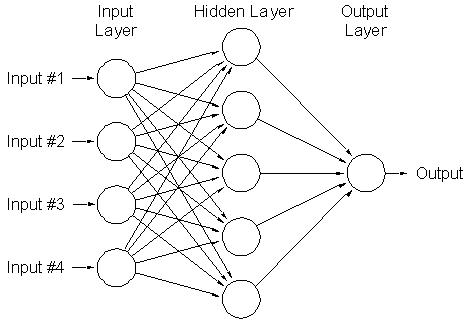
\includegraphics[scale = 0.3]{images/topology.png}
\end{center}
\caption{Topology of a feed-forward neural network\cite{Tan2006}}
\end{figure}

\section{Spiking Neural Network Simulators}

In order to give a better outlook on the field of spiking neural network simulation, this section will cover some of the state of the art solutions present to date.

\subsection{NeMo}

\emph{NeMo} is a spiking neural network simulator aimed at real-time simulation of large-scale neuron systems with the use of highly parallel GPUs.\cite{AndreasK.Fidjeland2009}
NeMo's main purpose is to produce simulations that would be particularly useful for research, therefore, main emphasis in this tool is put onto scalability and real-time aspects
of produced simulations.

NeMo is the main platform of MPI implementation for this project. The main goal is to improve inter-neural communication between computational clusters within NeMo.
At the same time, neuron mapping should be changed to ensure efficient communication during the simulation. NeMo simulator is going to be shown in more details in the following section.

\subsection{Brian}

Another solution, \emph{Brian} aims for bigger flexibility and ease of use, therefore making it more suitable for teaching purposes. \cite{Goodman2008} This
particular simulator will provide a good example of an spiking neural network simulator, and as it is easy to operate, will be useful for learning main concepts
of SNN in detail.

\subsection{SpikeNET}

\emph{SpikeNET} is a spiking neural network simulator created for large-scale integrate-and-fire networks simulations.\cite{ArnaudDelorme1999} As the main aim of this project is to
achieve the highest possible number of neurons hosted and computed simultaneously, this solution requires a very high level of parallelism in order to operate.
Therefore, findings from this project would be useful later in the project, when the focus is going to be on the scale of computations.

\subsection{Blue Brain Project}

Initiated in cooperation between IBM and EPFL, the \emph{Blue Brain Project} aims to produce a virtual brain in a supercomputer, Blue Gene, provided by IBM.\cite{BlueBrain} Computational power
required for the operations is immense, however, supercomputing technology gave neuroscientists a set of tools to solve this problem. The Blue Brain simulator is
a very interesting project, and due to exceptionally difficult task of reducing workload across the stations - it will be particularly useful at the stage of MPI development.

\section{NeMo Architecture}

The main project platform, NeMo, has most of its functionality concentrated around three classes - \emph{Configuration}, \emph{Network} and \emph{Simulation}.
ELABORATE


\section{Distributed Computing}

As the main objective of the project is to enhance communication efficiency between neurons in the spiking neural network, use of distributed computing plays crucial
role in its achieving. In this context, distributed computing means parallelization of tasks across the connected system and providing efficient communication medium
between separate computational clusters.

\subsection{Parallel Computing}

\emph{Parallel computing} is a form of computation where most of calculations are carried out simultaneously.\cite{G.S.Almasi1989} In order to achieve this, large problems
are divided into smaller independent parts that are carried out by separate computational units, with feeding the results either into the main cluster or holding it for further
computations. The rise of this particular field is due to the need in high-performance computing, especially in the light of frequency scaling becoming more and more
limited because of power consumption.\cite{Kumar2002}

Due to the nature of this project, a high degree of parallelism is crucial, in order to maintain the highest possible speed of simulation - the matter is that simulation would
be split between several clusters (\emph{nodes}) which, depending on the mapping, will operate independently, after receiving the information from main node at the start.
PICTURE

\subsection{Message Passing Interface}

\emph{Message Passing Interface} (MPI) is a language-independent protocol which acts as a communications medium for a group of processes.\cite{mpi} MPI's main function is to provide
a solid communication channel between the processes in a highly parallelised system, thus, enhancing efficiency of this system. Message passing programs are written in Fortran and 
C, with the use of built-in functions.

Currently NeMo has an MPI implementation within it, however, it is not the most optimal one. The main idea behind parallelisation in this project is that neurons are allocated, 
using mapping algorithm, between several computational nodes, which are communicating with each other with the use of MPI. Therefore, one of the main objectives will be to 
create an MPI layer inside system, that would increase the speed of computations by enhancing quality of inter-cluster communication.

There are currently several implementations of MPI to date, so here is a brief overview of available solutions.

\subsubsection{Open MPI}

The \emph{Open MPI Project} is an open-source implementation of MPI-2 maintained by a group of academic, research and industry partners, Open MPI Team.\cite{RichardL.Graham2005} This particular 
implementation aims at compatibility and high performance on all platforms, thus, making it quite easy to install and configure. Open MPI is a useful tool that will help understand 
the underlying concepts of message passing and generally give a good background within this subject area.

\subsubsection{MPICH2}

\emph{MPICH2} is an MPI implementation from Argonne National Laboratory, that aims at high performance and extendability.\cite{W.Gropp1999} The main idea of the project is to make the simulations as
fast as possible, via enhancing the efficiency of communication, therefore, MPICH2 fits well with the aims set, by providing focus on the speed and effectiveness. Another reason to choose 
MPICH2 for this project is that this package is already installed on the lab machines, therefore, saving time for the initial setup.\cite{W.Gropp1999a}

\subsection{Cluster-based approach and Mapping}

One of the most important part of the simulation is the initial \textbf{mapping} of neurons across the hosts, as it will affect the amount of inter-cluster communication and therefore overall efficiency of the system. \emph{Mapping} defines the layout of the resulting system and is directly affected by topology - neurons are split into several groups depending on the number of synapses connecting those. The main idea is to keep the amount of inter-cluster communication to minimum, as it is more expensive in terms of memory and time than communication within the node.

Mapping is defined by topology and hierarchy of the system - most of implementations have a master node, accountable for adding neurons and synapses to particular clusters, however, it is
possible to have a distributed system, were all nodes are equal in resposibility and actions are taken independently.

\subsubsection{Clustering algorithms and research}

Division of large scale networks, if applied correctly, greatly increases performance - making these nets computationally feasible to simulate. Consequently, there have already been several successful attempts of classifying best clustering algorithms. This section will give an insight into the algorithm introduced by Mark Newman which focuses on a specific parameter of the network - \emph{modularity}.

\textbf{Modularity} is a measure of the structure of the network that describes its strength of division into subgroups (\emph{modules})

\subsubsection{Current implementations of cluster-based approach within neural networks}
At the moment there are already a few implementations present that focus on the clusterisation of the neural networks in order to achieve better inter-neuron communication and bigger throughput. 
These are the most notable ones that have a direct connection to my project.

\begin{itemize}
\item{\textbf{Izhikevich's large scale model for simulating mammalian thalamocortical systems}}

The work by Eugene Izhikevich\cite{EugeneM.Izhikevich2008}, though being mostly focused on the research of brain dynamics, showed that clusterisation of the network system across several processors would result in much higher throughput rate for a large scale network - million of neurons, tens of millions of neuron compartmentss and almost half a billion synapses. In this particular case C with MPI implementation was used to allow for inter-cluster communication, and it allowed the researchers to scale the time needed for calculation of one sub-millisecond time-step for this type of network to one minute.

\item{\textbf{IBM cortical simulator project (C2)}}

Research conducted by a group of scientists from the IBM Research Centre in Almaden\cite{DharmendraS.Modha2007} focused on creation of a platform capable of simulating cerebral cortex activity. Consequently, due to extremely large scale of simulation - in this project more than 55 million Izhikevich neurons were simulated within one network - and availability of clusters within the centre, a distributed approach was applied with the use of MPI. When applied to this problem, cluster mapping managed to achieve balanced workload across the network, as well as the uniform inhibitory neuron distribution. The reason the latter point mattered in the simulation is the fact that more than 60\% of firing was inhibitory - therefore, incorrectly distributed neuron set would have a significant effect on results.

\item{\textbf{Neuromorphic model for GPGPU cluster}}

Simulator produced by Bing Han and Tarek Taha aimed at the speedup of simulations with Izhikevich and Hodgkin-Huxley neuron models\cite{TarekM.Taha2010}. Use of GPGPUs and multi-threaded MPI provided heterogeneous  clusters and per-cluster computational capacity, and clustering algorithm ensured correct distribution of neurons in accordance to the 2 layers present in the system. As a result, a significant speedup was achieved in computation, factor of 177.0 for Hodgkin-Huxley and 24.6 for Izhikevich neurons, for the task of image recognition.
\end{itemize}


\chapter{Objectives and Design}

This chapter will provide the overview of the goals set by the project, design implementation aimed to meet those and certain properties of the problem that affected the solution.
It will also cover design paradigms used for project guidance, as well as, the set of tools used for outlining its aspects.

\section{Main Objectives}

Throughout the course of project, the main aims that were targeted had been:

\begin{itemize}
\item {\textbf{Create a distributed version of NeMo, making it capable of scalable simulations with the use of multiple processes}}
\item {\textbf{Throughout implementation of the distributed capabilities, leave the core NeMo functionality intact - build on top}}
\item {\textbf{Implement clustering algorithm that would allow the resulting program to operate within the network capacity and distribute the workload in a more efficient manner}}
\item {\textbf{Lower the requirements set by the platform for the target machine(s) through parallelization}}
\end{itemize}

Setting out the objectives this way helped to percieve a more detailed picture of the project as a whole and gave understanding of the set of stages that were to be accomplished in order to
make the project meet these objectives.

\section{Objective-specific Structure}

After having all of the main goals set out, it is important to get the structure of the design, with focus on satisfying these goals. In this section, the design focused on each of the features of the project will be discussed.

\subsection{Distributed Version of the Simulator}

In order to provide a more detailed picture of the distributed system, here is the set of inner classes of the NeMo core simulation classes.

PICTURE

Creation of the distributed system that would run the simulator could be split into 3 distinct steps:

\begin{enumerate}

\item{\textbf{Creation of fully separate homogeneous simulation}}

By accomplishment of this step, the system has to be able to run on several processes with little input from the user and no interaction between processes within simulation - in other words, several separate NeMo simulations with their own self-generated parameters, that could be started by user signal from the main process.

\begin{figure}[h]
\begin{center}
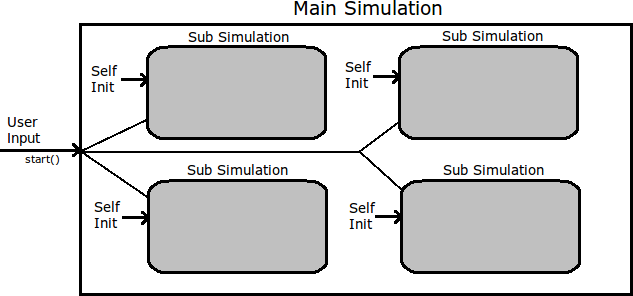
\includegraphics[scale = 0.25]{images/design_stage_1.png}
\end{center}
\caption{Schematic model of step 1}
\end{figure}

\item{\textbf{Integrating the initialisation parameters distribution across the network}}

After thorough research conducted into the use of MPI protocol, create a simulation that would encode and pass all the initialisation parameters to the networks - mapping, configuration, neuron and synapse data - however, still without interaction between the sub-simulations.

\begin{figure}[h]
\begin{center}
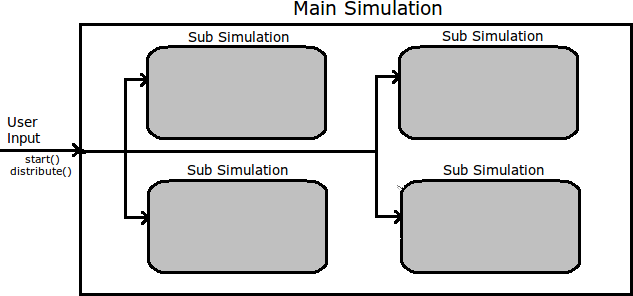
\includegraphics[scale = 0.25]{images/design_stage_2.png}
\end{center}
\caption{Schematic model of step 2}
\end{figure}

\item{\textbf{Implementation of the full non-constrained communication between the nodes within the network}}

Having the basic distribution system created, integrate the inter-node communication system that would allow subsystems to pass the internal spike data during simulations, while main class synchronizes the steps of all simulations by
waiting for all of the communication to end, and advancing simulation one step further.

\begin{figure}[h]
\begin{center}
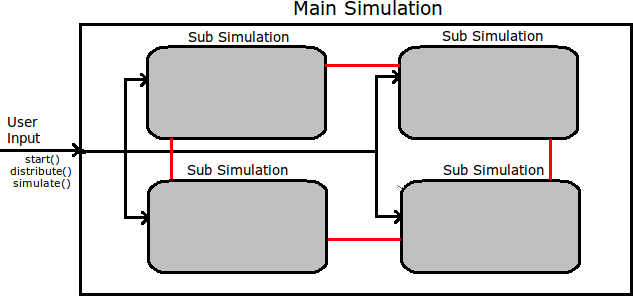
\includegraphics[scale = 0.25]{images/design_stage_3.png}
\end{center}
\caption{Schematic model of step 2}
\end{figure}

\end{enumerate}

Accomplishing all of these steps yields a fully working distributed implementation of the target system. It is worth noting that though this design is quite schematic, the results of the actual implementation if broken into steps were closely related to those presented by this plan.

\subsection{Separation from the Core System}

\begin{figure}[h]
\begin{center}

\includegraphics[scale = 0.1]{images/placeholder.jpg}
\end{center}
\caption{NeMo simulation core}
\end{figure}

These classes is the core of the NeMo functionality, as it comprises all the data sets needed for the correct simulation. Therefore, in order to enable the distributed version to run separately, i.e. without interfering with the data innate to these classes, it is essential to design the system around those. In other words, the correct design must not alter internal structure of this set of classes.

\begin{figure}[h]
\begin{center}

\includegraphics[scale = 0.1]{images/placeholder.jpg}
\end{center}
\caption{Distributed simulation design}
\end{figure}

As it can be easily observed, the distributed version treats the core simulation classes as separate entities, only interacting with them through the NeMo-specified functionality and set of public methods, already present in them.
Objectively, the MPI Layer wraps around the simulation classes and enables communication by passing input and output data between separate NeMo simulations.

\subsection{Mapping}

\begin{figure}[h]
\begin{center}

\includegraphics[scale = 0.1]{images/placeholder.jpg}
\end{center}
\caption{Mapping scheme}
\end{figure}

\subsection{Alternative Solutions}
\begin{itemize}

\item {Latency and Spike delivery}

Due to latency within the network of processors the system was tested on, there were a few precedents of race conditions that caused uncertain behaviour of the simulator - therefore, giving output that differed significantly from the desired one. In order to overcome this drawback, a timer system within the master simulation has been implemented - this ensured control of the communications, and allowed for stops with delay, to deal with propagating spikes. That move has significantly increased precision of the simulation, moreover, giving a better overview of the performance.

\end{itemize}


\section{Final Design}

\section{Tools}


\chapter{Implementation}

This chapter will cover the actual implementation of the project. The whole process of implementation was split into two parts: creation of the MPI Layer and clustering implementation within the Mapper class.

\section{MPI Layer}

The MPI Layer, as mentioned before, operates, based on the two main entities - \textbf{MasterSimulation} and \textbf{WorkerSimulation} classes.

\emph{MasterSimulation} is responsible for clustering and separation of the user input, distribution of this information to the corresponding workers and synchronisation of workers during simulation timesteps. It is the core class of the simulation, as it receives original network parameters, specified by the user.

\emph{WorkerSimulation} (sometimes regarded as nodes) is running the simulation and communicates with Master, to receive user-input information (initialisation parameters), and with other Workers during simulation. This is an auxiliary class, that is fully responsible for the local NeMo simulation running on its cluster.

\subsection{Basic Distributed Platform}

The construction of the basic platform focused on establishing the communication channel between the master simulation and the worker ones. This meant MPI initialisation on both sides, followed by an exchange messages with commonly known communication tags.

The earliest version of the distributed system, that implemented the first design step of building a distributed simulation, consisted of a master, sending out one integer (in this case it was number of neurons to be simulated), that was received by all workers. Once they received this message, self-initialisation of all parameters of the simulation followed, with consequent asynchronous completion after a set number of steps.

\subsubsection{Initial parameters distribution}

Having this initial setup ready, implementation of the second step of distributed version creation followed.
The master simulation, after having both Configuration and Network passed to it, did a basic division of the neurons per worker - distributed those uniformly (until the Mapper is fully implemented):
\begin{equation}N_{per\ worker} = \frac{N_{neurons}}{N_{workers}}\end{equation}
The translation of global id to a local one implemented within mapper at that stage is also simple:
\begin{equation}ID_{global} = ID_{local} + (Rank_{worker}-1)*N_{per\ worker}\end{equation}

\begin{figure}[h]
\begin{center}
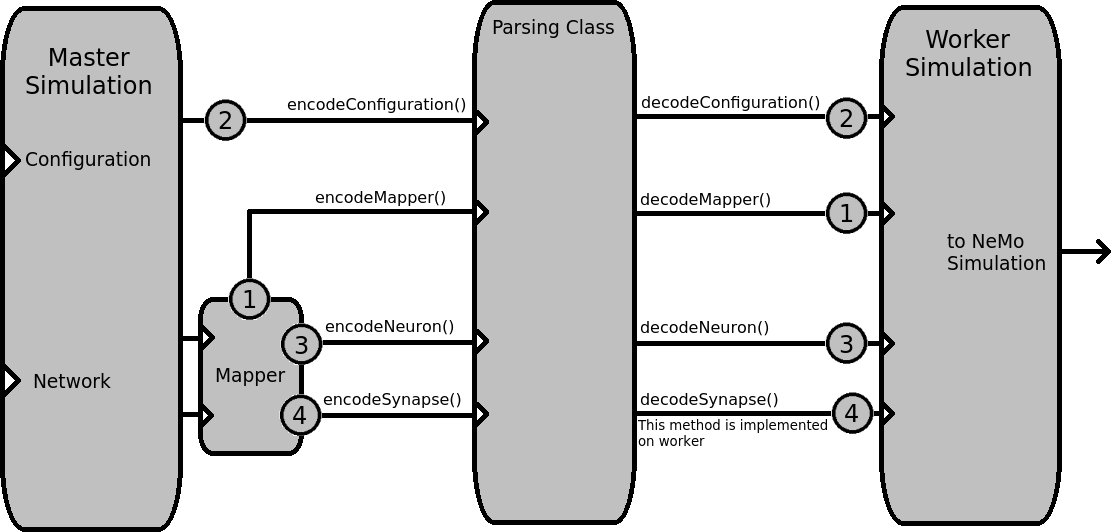
\includegraphics[scale = 0.5]{images/implementation/distribution.png}
\end{center}
\caption{Parameters distribution}
\end{figure}

Once the worker set of parameters needed for initialisation was finalised, those need to be encoded and sent out to the workers. This is done through a set of parsing methods - a pair encode-decode for each type of the data. If the data sent is heterogeneous, i.e. more than one primitive datatype is present, the information is encoded into a string of values.

Parsing class was added for the encoding and decoding capabilities - it is accessible by both Master and Worker classes. It provides set of methods for encoding and parsing messages for further use during MPI calls.

The whole distribution stage can be split into 4 distinct steps:

\begin{enumerate}
\item{\textbf{Mapper distribution}}

Mapper has to be encoded with all information present inside - all workers must have the same mapping to ensure correctness of later communication. The data sent is split into a number of strings corresponding to the number of workers and broadcasted for the consequent reconstruction on the sub-simulation.

\item{\textbf{Configuration distribution}}

Configuration is encoded into a string that is also broadcasted to all workers. The information passed does not change, therefore, there is no need to iterate through each master-worker channel.

\item{\textbf{Neuron distribution}}

Once the mapping is set up, the neurons are distributed according to it. Firstly, the worker receives the number of neurons, and then MPI receive method is looped to gather neuronal data. Every string received is decoded, the global index is mapped locally, and, once it is done, a new neuron with this set of parameters is added to the local network.

\item{\textbf{Synapse distribution}}

The last part of the distribution stage, synaptic distribution, is also the most complex - the internal (both source and target are on the same node) synapses are sent as strings to the corresponding worker, whereas external ones need indication for the external target or source. This is done through assigning a negative value to them:
\begin{equation}Value_{external} = -(Value_{internal}+1)\end{equation}

Worker simulations have two data structures for storing incoming and outgoing synapses. The latter is built simply as an array of pairs - local id of a neuron and a vector of targets. The former, however, needs to store the synapse data - local target, weight, delay, plasticity - so it is structured as a vector of vectors of structs. These two are populated as the worker receives and decodes the synaptic data for external synapses.

Note, that even though the external synaptic structure was implemented, it is not put to use at this stage, as there is no spike delivery integrated between sub-simulations within the system at this point.
\end{enumerate}

Once all parameters are received, workers set up their simulations and notify master when it is done. When master receives confirmation from all workers, the simulation may commence, through broadcasting the step signal across the network. 

\subsection{Communication Channels Integration}

At this point the system has a fully operational master-worker distribution channel. Next step is implementation of an inter-worker communication channel used for spike delivery.

First of all, the sources need to be identified, to acquire knowledge of the corresponding targets and their worker location. As given by the NeMo architecture, the simulation step function returns IDs of the neurons fired during this simulation step. These are then used to derive any outgoing spikes, i.e. going through external synapses. The worker step function is done in similar way to the original NeMo implementation, it could be split into three sub-steps\cite{AndreasK.Fidjeland2009}:

\begin{enumerate}
\item {\textbf{Enqueuing Spikes (Prefire)}} 

This is a stage during which the data about incoming currents is collected and passed to the fire function.
Within MPI Simulation, function $enqueueIncomingSpikes()$ provides this functionality, by taking the incoming current data and passing it to the NeMo simulation $step()$ function.

\item {\textbf{Local Simulation Step (Fire)}}

This function determines which neurons have fired by updating the neuron values based on the data collected during prefire step. Original NeMo simulation $step()$ function is used as \emph{Fire} stage returning the vector of fired neurons. The fired neurons are passed to the postfire function.

\item {\textbf{Distributing Spikes (Postire)}}

The final stage of the simulation step, during which the spikes are distributed across the network. Local distribution is done within NeMo step, external is done through series of MPI calls by Worker simulations.
\end{enumerate}

Once a Worker has finished its step, it sends notification to the Master, who, after receiving confirmation from all Workers, advances the global simulation one step further.

After finalisation of overall communication structure, the external delivery design needs to be specified. In the following sections the spike delivery system is given in details.

\subsubsection{Spike Enqueuing}

In order to provide the capacity of storing the incoming spikes, WorkerSimulation class has two data structure for storing those: dequeuing $incoming\_queue$ and priority $delay\_queue$.

The purpose of $incoming\_queue$ is to collect global IDs of all neurons, that have a target on this node. It is populated during the later distribution step.

The $delay\_queue$ is created to store the spikes depending on their delay values. Delay represents number of simulation steps that need to commence before this spike reaches the target node.

\begin{figure}[h]
\begin{center}
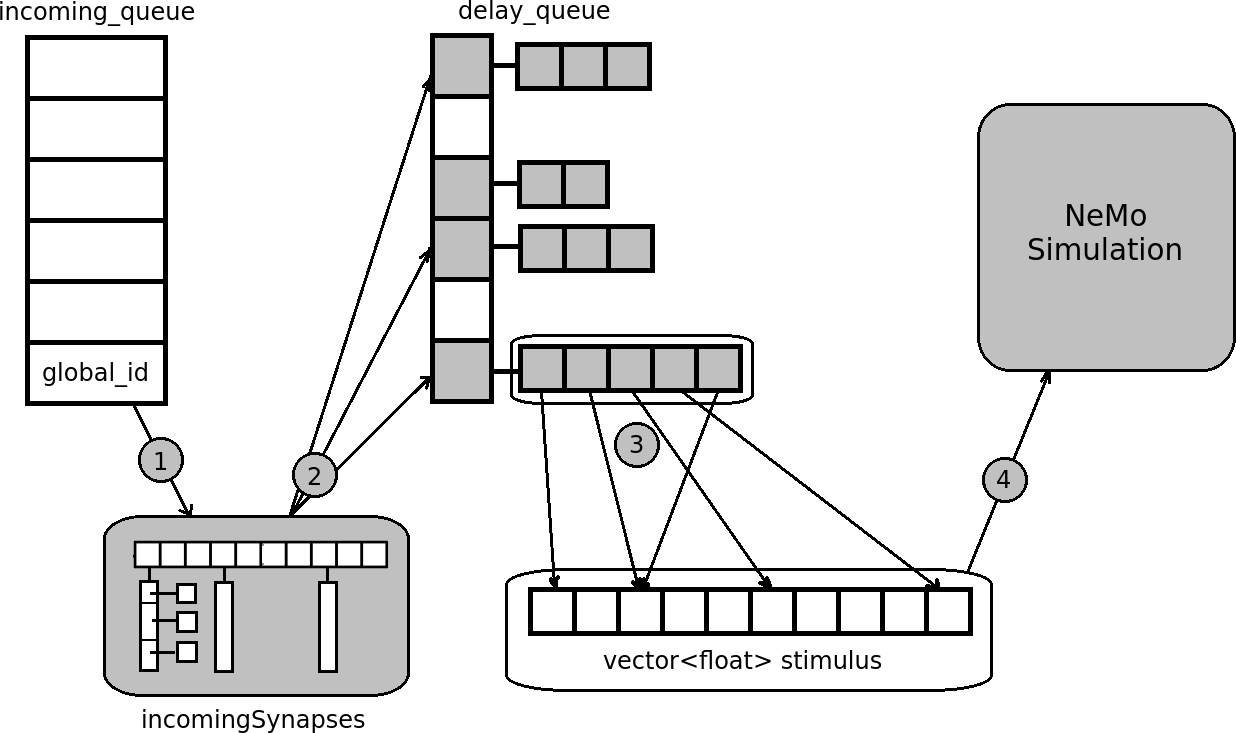
\includegraphics[scale = 0.5]{images/implementation/spike_enqueuing_scheme.png}
\end{center}
\caption{Representation of spike enqueuing}
\end{figure}

Taking this into account, $enqueueIncomingSpikes()$ function can be split into two steps:

During first step, it continously dequeues $incoming\_queue$ (1), while it is not empty, looks up the targets connected to this source in Worker's $incomingSynapses$ structure, and puts them into $delay\_queue$ depending on their delays (2). 

The second step commences, after the delay sorting has been resolved. A vector of floats (incoming currents) $stimulus$ is initialised with size corresponding to the number of neurons on the node and values set to 0.0. The head of the delay queue (delay = 1) is poped and iterated through (3). Each entry consists 2 values: target and weight. Using those, the current vector is updated: for each target a synapse weight is added to its current value (4).

The resulting vector is then passed to the local NeMo simulation $step(stimulus)$ function.

\subsubsection{Spike Distribution}

The simulation step returns a vector $fired$ of local neuron IDs, indicating the neurons that have fired. After taking this vector as a parameter, $distributeOutgoingSpikes(fired)$ performs external distribution of spikes.

\begin{figure}[h]
\begin{center}
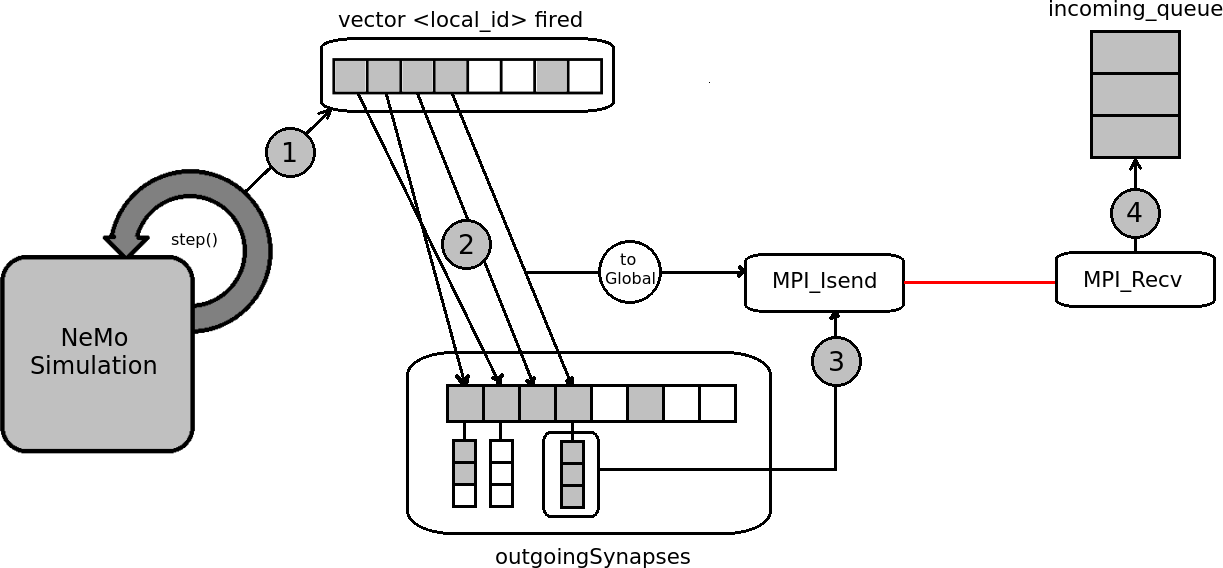
\includegraphics[scale = 0.5]{images/implementation/spike_distribution_scheme.png}
\end{center}
\caption{Representation of spike distribution}
\end{figure}

This function can also be split into two steps:

First step: the vector of fired neurons (1) is iterated through, IDs are looked up in the $outgoingSynapses$ structure. As each ID has a vector of corresponding target nodes (2), this vector is iterated through (3), and a non-blocking MPI message with the global ID of a neuron is sent to the target. After the distribution is finalised, an ending message is sent to all workers.

Second step: after all non-blocking messages have been sent, function initiates a loop that enqueues (4) all incoming IDs into the $incoming\_queue$. This loop only terminates after receiving the ending messages from all other workers.

After finishing these two steps, the function returns, leading to the end of the distributed simulation step on this worker.

\section{Clustering}

Clustering implementation is dependent on the algorithm introduced by Mark Newman in 2006. This section will provide the mathematical overview of this algorithm and its implementation within Mapper class.

\subsection{Newman's Algorithm}

Major part of Newman's research concentrates on finding communities in the network structures\cite{NewmanComm}. \emph{Community structure} is a feature of a graph that shows the gathering of vertices into groups with high connectivity. This feature is best described by modularity, the measure of modular division of a particular network into subnets with high edge density.

Formula for modularity is (for a network of $n$ vertices):
\begin{equation}Q = \frac{1}{4m}\Sigma_{ij}(A_{ij} - \frac{k_{i}k_{j}}{2m})s_{i}s_{j}\end{equation}\cite{Newman2006}
where $m$ is total number of edges, $k_{i}$ and $k_{j}$ are the degrees of the corresponding neurons. Notice that $\frac{1}{4m}$ is a conventional leading factor - it is there to support previous definition of modularity, given by Newman and Girvan\cite{Newman2004}.

Newman's algorithm ("Method of Optimal Modularity"\cite{Newman2006}) is a way of determining the natural division of graph's vertices into several non-overlapping communities, based on the modularity measure. Its structure is different to the older algorithm used for finding communities\cite{NewmanAlgo}, as the latter was more scientifically focused, therefore lacked certain capabilities for implementation in the parallel computation design.

The step structure of the algorithm is as follows:

\begin{enumerate}
\item{\textbf{Create an adjancency matrix of the network}}

Create and populate the adjacency matrix for the network based on the information about edges.

\item{\textbf{Create and populate a modularity matrix of the network}}

Matrix $Q$ is created with the same dimensions as the adjacency one. Its values are set through using equation:

\begin{equation}Q[i][j] = A[i][j] - \frac{k_{i}k_{j}}{2m}\end{equation}

Notice that the conventional factor is abolished - it does not affect the result, so its absence will improve execution time.

\item{\textbf{Generate a leading eigenvector for the modularity matrix}}

For the resulting Q matrix the dominating eigen vector has to be generated - this is done through the use of power-iteration algorithm\cite{VonMises1929}.

Power iteration algorithm: $b_{k+1} = \frac{Ab}{||Ab||}$

\item{\textbf{Eigenvector values are used to split the network into two partitions}}

The values of eigenvector correspond to the split of this network into two parts - negative and positive values separate vertices into two groups. In case, more groups are needed, the algorithm is performed again on the partitions.

\end{enumerate}

As it can be observed Newman's algorithm is robust and relatively easy to implement. Moreover, it possesses another feature - whenever the connectivity of the network is all-to-all or close to this state, the resulting eigenvector would have only positive values - therefore, indicating an indivisible graph, i.e. a graph without a natural community separation. This certain feature could be used later for improvement - specifically for the purpose of finding an optimal number of clusters that a particular network has to be split into.

\subsection{Mapper integration}

The implementation of Newman's algorithm into the Mapper class is essentially translation of all of the algorithmic steps into the code. The focus, therefore, should be on the matrix updates and the power-iteration function.

The main difference from the actual algorithm would be the use of one matrix instead of two - this is done to prevent probable memory leaks, as testing with large scale networks showed that matrices for big number of neurons occupy too much RAM, causing the Master process to get killed. Therefore, current implementation has a threshold value of 31000 neurons, after which a simple uniform distribution is used for clustering.

This is the implementation of adjancency and modularity (both within $q\_matrix$) update.

\begin{center}
\lstset{
    caption = Code for Matrix update,
    basicstyle=\ttfamily\footnotesize\bfseries,
    frame=tb
}
\begin{lstlisting}
...
/* Parameters initialisation */
for(i = 0; i < ncount; ++i) {
	vector<synapse_id> synapses = net.getSynapsesFrom(partition[i]);
	for (j = 0; j < synapses.size(); ++j) {
		unsigned globtarget = net.getSynapseTarget(synapses[j]);
		if (auxMap[globtarget] == partcount) {
			unsigned target = backMap[globtarget];
			q_matrix[i][target]++;
			q_matrix[target][i]++;
			degrees[i]++;
			degrees[target]++;
			edges++;
		}
	}
}
for (i = 0; i < ncount; ++i) {
	for (j = 0; j < ncount; ++j) {
		if (i != j) q_matrix[i][j] = (q_matrix[i][j] - (float)(degrees[i]*degrees[j])/(2*edges));
		else q_matrix[i][j] = STRENGTH;
	}
}
\end{lstlisting}
\end{center}

In the code shown above, the first loop initialises the adjacency matrix - it is done through interaction with the Network class. For each of the synapses, source and target values are checked to be within the partition. Once proved to be correct, values for adjacency, degree of vertices and number of edges are updated.

The second loop constructs modularity matrix on top of the adjacency one. The updates are done in accordance to the modularity formula, mentioned before (4.5).
The constant STRENGTH is set for all $q\_matrix_{ii}$ objects for the purpose of better computations, as original algorithm did not permit loops.
Also, note that due to big size of all created data structures, each call for $allocateNeurons()$ is ending with a set of destructors.

Once the $q\_matrix$ values are all set, the only thing left to do - is to calculate the dominant eigen vector of this matrix:

\begin{center}
\lstset{
    caption = Power-Iteration (Von Moses) algorithm,
    basicstyle=\ttfamily\footnotesize\bfseries,
    frame=tb
}
\begin{lstlisting}
float* eigenvector = new float [ncount];
float* tmp = new float [ncount];
...
/* Parameters initialisation */
while(step < THRESHOLD) {
	norm_sq=0;
	for (i = 0; i < ncount; ++i) {
        	tmp[i] = 0;
       		for (j = 0; j < ncount; ++j) tmp[i] += q_matrix[i][j] * eigenvector[j];
		norm_sq += tmp[i]*tmp[i];
	}
   	norm = sqrt(norm_sq);
	for (i = 0; i < ncount; ++i) eigenvector[i] = tmp[i]/norm;
	step++;
}
\end{lstlisting}
\end{center}

This part of code is responsible for the eigen vector generation. Eigenvector is first set to {$1,1...1$} and then passed to the while loop for several steps of power iteration. The number of steps, THRESHOLD constant, after thorough testing, is set to 10, as this number of iteration steps provides a compromise between accuracy and heaviness of computation.

\begin{figure}[h]
\begin{center}
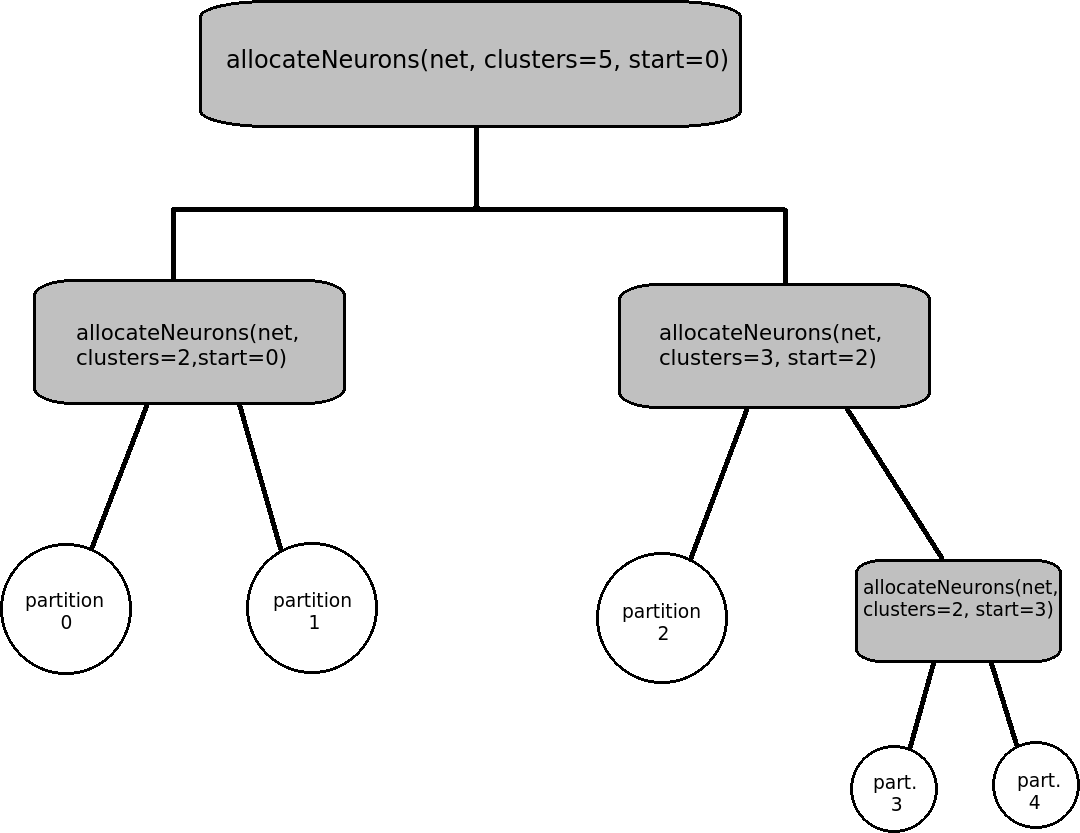
\includegraphics[scale = 0.4]{images/implementation/clustering_recursive.png}
\end{center}
\caption{Representation of a recursive call to the clustering function for 5 clusters}
\end{figure}

\clearpage

\section{Alternative Solutions}

There were a few alternative ways that the above algorithms could be implemented - however, most of them quickly proved to be insufficient for the purpose or too time-consuming to implement.

\begin{itemize}
\item{\textbf{Use of Boost MPI libraries}}

The idea of this solution was that boost MPI libraries comprise all needed functionality in an easy and well-represented way. However, use of both Boost and CMake caused numerous build fails, which in the end, outweighed the positive side. Moreover, most of the system that was implemented already at that point was written with MPICH - therefore, a change of implementation library would consume more time.

\item{\textbf{Implementation of spike receiving into enqueuing step}}

This proposal was aimed at having a wider window of simulation - by creating unblocking receives at the start, that would be filled in with the non-blocking send. However, such an implementation is leading to race conditions occuring, and, moreover, needs the starting input sent from all nodes, which could cause a significant overhead. Furthermore, a single communication window implemented in $distributeOutgoingSpikes()$ method is much easier to control and debug, whenever an MPI call fails.

\item{\textbf{Expand the limits of mapping by using both uniform and Newman clustering algorithms}}

As mentioned before, the current implementation of clustering algorithm is not fully applicable to large scale networks, mostly due to the RAM limitations. However, uniform mapping does not require that much memory, therefore, if it is done first, leaving less computationally heavy chunks for advanced clustering, it should produce faster results. The outcome however, is quite the opposite - the initial uniform distribution adds the most external synapses to the partitions - as a result, rendering most of the further clustering not as useful, especially considering setup time spent on it.
\end{itemize}


\chapter{Evaluation}

After full implementation of the design proposed to the project, there has to be careful evaluation of the outcomes, or more specifically improvements introduced by such an implementation. At this point the distributed version with built-in clustering is fully developed, and the focus is on the possible criteria of the resulting product evaluation.

\section{Current Solutions}

There are already quite a few projects within the area of distributed neural network simulation. Here are some that are most similar in structure with the current project (most of them were mentioned in the Background section).

\subsection{Blue Brain Project}

The Blue Brain Project initiated in collaboration by IBM and EPFL, is aimed to reconstruct the virtual brain on the BlueGene/L supercomputer.\cite{BlueBrain} This project set its objectives in simulating the real virtual brain, as it has already succeded the simulation of a rat cortex. With the sheer numbers of neurons present in simulation closing to $10^9$, this is the project with the most resource power among listed here.

\subsection{SpikeNET}

The SpikeNET simulator focuses on the scalability of the simulation - it is concentrated on simulation of large number of integrate-and-fire neurons which spikes are computed in parallel\cite{ArnaudDelorme1999}. For most parts of its implementation SpikeNET is quite similar to the NeMo project. However, its parallel computation implementation does not exploit a fully distributed parallelism, i.e. most of computation still lies within the scope of one process.

\subsection{OpenSim}

The OpenSim project on the other hand, relies on distribution of neural simulation into a set of parallelizable sub-tasks across a cluster of machines\cite{OpenSim}. However, due to the age of its most recent implementation, the techniques used within it might already be outdated, as more efficient communication channels were developed. Nevertheless, OpenSim, due to the fact that it relies on a fully distributed system, has many similarities in structure with this project. \\ \\


Even though, all of these projects could be compared against the MPI NeMo, the differences between the implementations alone will not be sufficient to make a fully informed judgement. The problem is the lack of common ground - all of these implementations vary in the ways of neuron representation, SpikeNET lacks delay functionality and Blue Brain is built on the platform which resource base cannot be challenged by the resources of NeMo project.

Therefore, a much more sensible approach would be to compare the current version of distributed system against the "clean" NeMo version and see which particular points of simulation are different between those two.

\clearpage

\section{Criteria of Comparison}

As the test platforms are chosen, it is time to pick a set of criterias which will tested to produce informative results. In order to pick the most informative criteria, there has to be an insight into the main variables within simulation. Those are:

\begin{itemize}
\item{\textbf{Setup Time}}

This criteria comprises the temporal requirements for the simulation to be set up in order to be run. Within core NeMo functionality, this time would be comprised of the simulation setup time which is almost negligible, since the Network object constructed, operates within Simulation. For the distributed system, however, startup time is split differently: it includes the clustering time and initialisation parameters distribution window - which could be further split into 4 steps - mapper, configuration, neurons and synapses.

\item{\textbf{Simulation Time}}

The simulation time is a measure of the simulator performance according to the time spent on the actual simulation; the variables that are set for the simulations are:

\begin{enumerate}	
	\item{Number of neurons} within the network
	\item{Number of synapses per neuron}
	\item{Number of simulation steps} - constraint put on the number of simulation steps to derive time requirement per step.
\end{enumerate}

Therefore, by iterating through each of these variables, while keeping others constant, it is possible to get the dependency of the current implementation on the particular parameter, and how its value affects the overall simulation.

\item{\textbf{Network throughput}}

Last criteria that could also represent the network - total spiking within network during simulation. This value highly depends on the number of neurons and the overall interconnectivity - the current implementation would only show the number of fired neurons and external spike deliveries.

\end{itemize}

Having set out all of the meaningful criteria, it is time to look at them in detail and compare the data gathered with different systems.

\section{Setup Time}

This section will cover the simulation setup stage of the distributed system's initialisation.

\subsubsection{MPI clustering and distribution overhead}

\begin{figure}[h]
\begin{center}
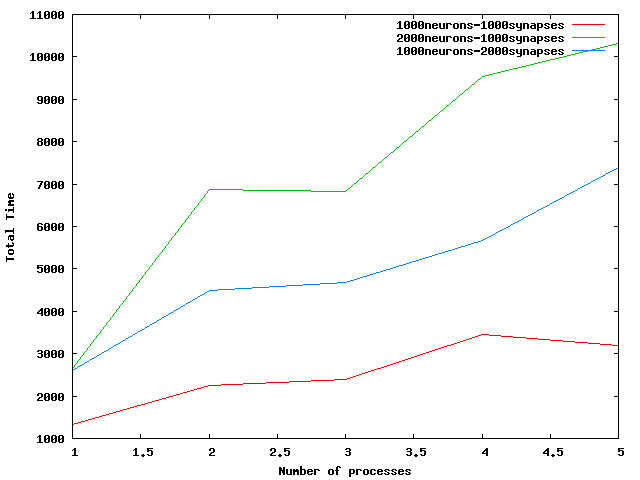
\includegraphics[scale = 0.5]{images/evaluation/setup_comparison.png}
\end{center}
\caption{Comparison of setup time to the number of neurons, synapses and processes}
\end{figure}

From the above graph it is easily observable that the most amplifying factor for simulation setup time is the number of neurons. The setup time, however, can be further split into the 5 times - clustering, mapper, configuration, neuronal and synaptic distributions.

The ones having the most effect on the simulation setup time are clustering and synaptic distribution. Now, if those are observed closer under particular circumstances, their dependance upon other variables is clearly seen:

\begin{figure}[ht]
\begin{minipage}[b]{0.5\linewidth}
\centering
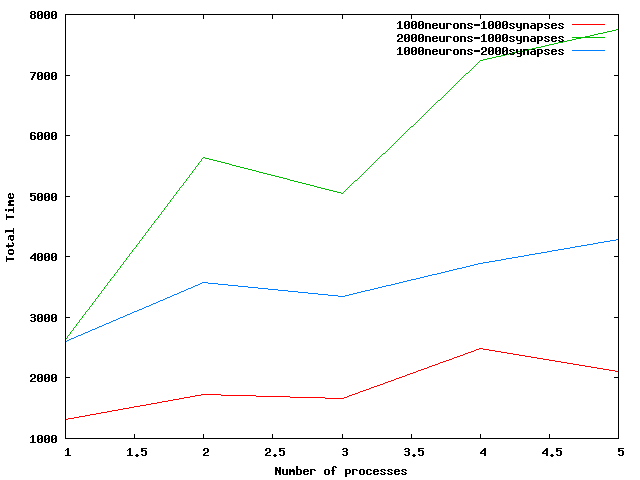
\includegraphics[width=\textwidth]{images/evaluation/syndistr.png}
\caption{Synaptic distribution}
\label{fig:figure1}
\end{minipage}
\hspace{0.5cm}
\begin{minipage}[b]{0.5\linewidth}
\centering
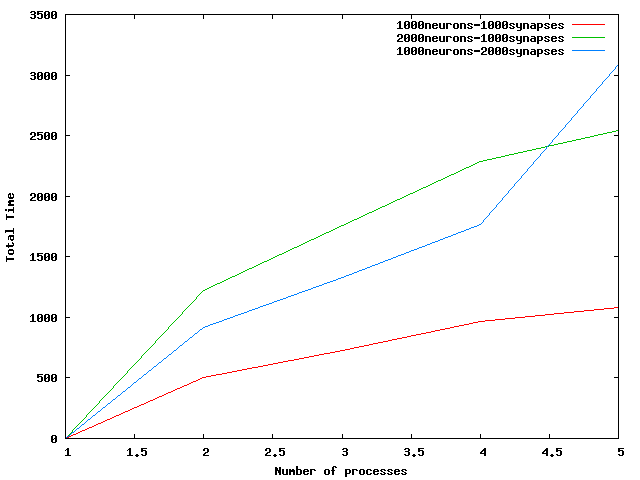
\includegraphics[width=\textwidth]{images/evaluation/cluster.png}
\caption{Clustering}
\label{fig:figure2}
\end{minipage}
\end{figure}

From these graphs, it can be concluded that synaptic distribution depends more on the number of neurons and workers rather than on the per-neuron synapse count. As for the clustering, its timeline correlates with the increase in the number of processes - which is logically correct, since this means more calls to the clustering function at the startup.

\section{Simulation Time}

This section attempts evaluate the collected results of running multiple distributed simulations against the original NeMo simulation, and show the particular differences through simulation running time. The results of this evaluation show that even though the system has been implemented, there is still much more work on its optimisation.

\subsection{Number of neurons}

\begin{figure}[h!]
\begin{center}
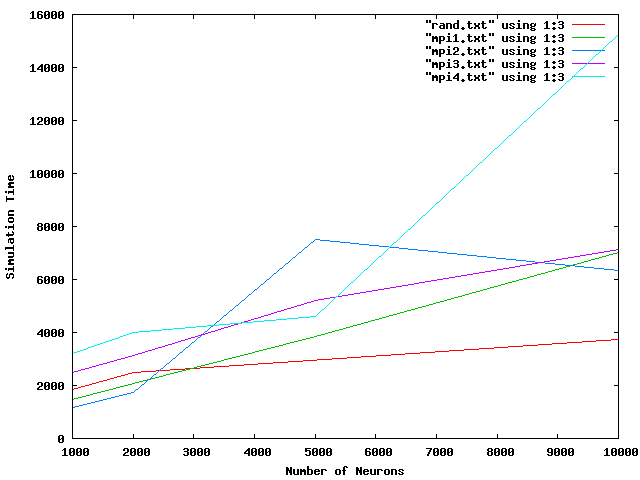
\includegraphics[scale = 0.4]{images/evaluation/distributed_neurons.png}
\end{center}
\caption{Comparison of setup time to the number of neurons, synapses and processes}
\end{figure}

The set constants: synapses = 1000, steps = 5000.

This comparison graph shows that from the point of performance, the distributed version does not lose much of its potential - the communication overhead does not highly correlate with the number of neurons. Therefore, potentially for a simulation of a much larger scale, the graph for a distributed simulation of 3 processes would go below the original NeMo graph. The reason for this proposition is that as the number of neurons grows the time taken for a simulation step on a single NeMo implementation grows with a factor of this increase. On the other hand, the distributed version has a more fixed value of growth, and at the same time, the local simulations, depending on the number of clusters are much more computationally feasible as opposed to having one big simulation.

\subsection{Number of synapses}

\begin{figure}[h!]
\begin{center}
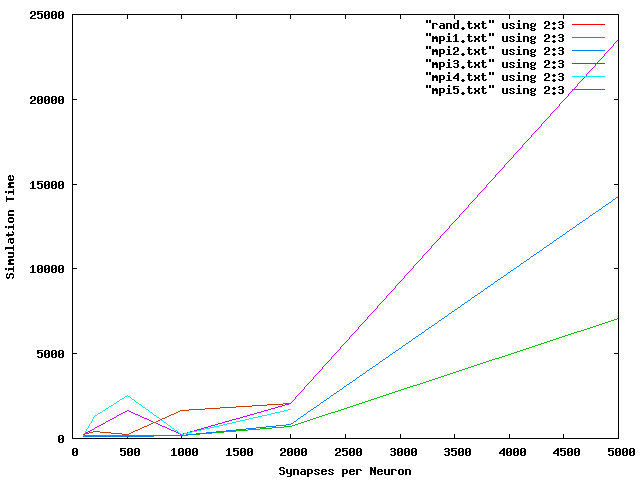
\includegraphics[scale = 0.4]{images/evaluation/distributed_synapses.png}
\end{center}
\caption{Comparison of setup time to the number of neurons, synapses and processes}
\end{figure}

The set constants: neurons = 2000, steps = 500.

This graph shows that synaptic density per neuron dramatically affects the external spike delivery. Even with the mapping algorithm implemented, the number of spikes fired is still difficult to handle within one simulation step. This particular set of results suggests that there could be much more work done on the inter-nodal communication engine. The graph could also suggest poor choice of constants, as the scope of this simulation is far too small to see the real impact of the distributed simulation. Therefore, potentially, a further set of measurements should be taken to provide a better overall picture.

\subsection{Number of steps}

\begin{figure}[h!]
\begin{center}
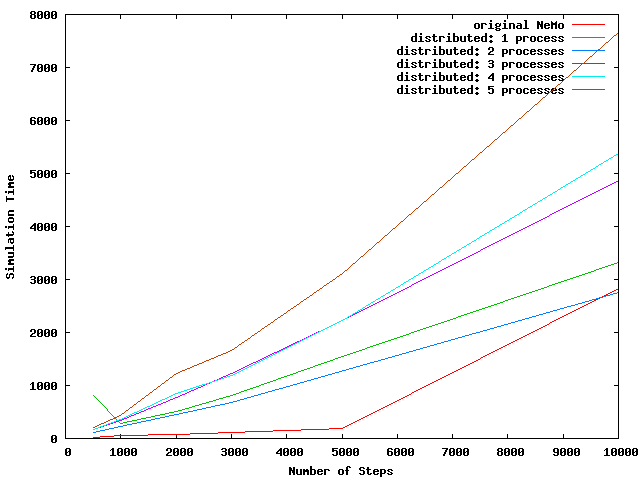
\includegraphics[scale = 0.4]{images/evaluation/distributed_steps.png}
\end{center}
\caption{Comparison of setup time to the number of neurons, synapses and processes}
\end{figure}

The set constants: neurons = 1000, synapses = 1000.

Through the graph of steps against simulation time it can be easily observed that distributed implementation has a constant per-step time. At the same time the simulation time for the original NeMo simulation went up significantly with the number of steps. This could in turn suggest that as the simulation progresses the number of spikes increases dramatically, causing the decrease in speed of the NeMo simulation. Therefore, if mapping is correctly implemented, as simulation progresses the work that has to be done would be significantly smaller on the sub-simulations, and the external spike delivery will not be ruined by the sudden peaks.

\clearpage

\section{Network throughput during simulation}

\begin{figure}[ht]
\begin{minipage}[b]{0.5\linewidth}
\centering
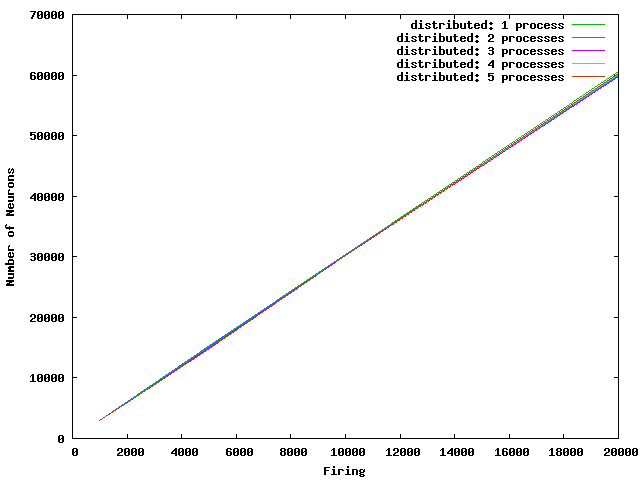
\includegraphics[width=\textwidth]{images/evaluation/neuron_firing.png}
\caption{Neuron number against firing}
\label{fig:figure1}
\end{minipage}
\begin{minipage}[b]{0.5\linewidth}
\centering
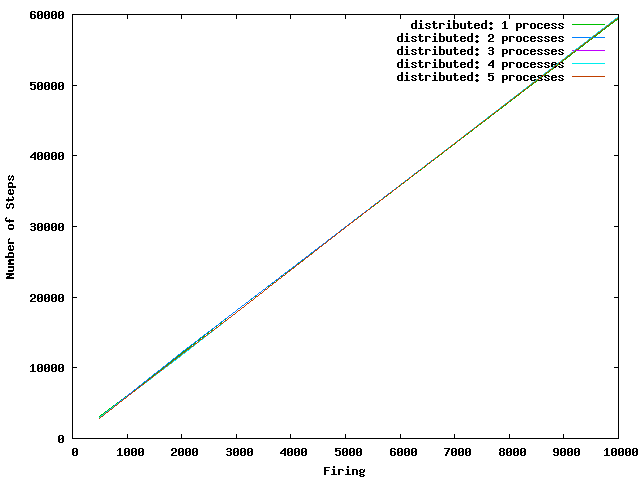
\includegraphics[width=\textwidth]{images/evaluation/steps_firing.png}
\caption{Number of steps against firing}
\label{fig:figure3}
\end{minipage}
\end{figure}

These two figures show linear proportionality - amount of firing is directly proportional to the number of neurons and number of steps.
The third figure, however, gives a slightly different information. It shows that the synaptic density is not directly proportional to firing capacity.

\begin{figure}[h!]
\begin{center}
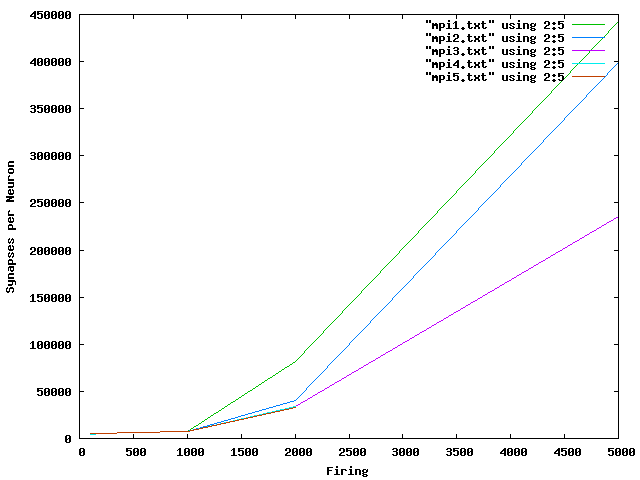
\includegraphics[scale = 0.5]{images/evaluation/synapses_firing.png}
\end{center}
\caption{Synaptic density against firing}
\end{figure}





\chapter{Conclusion}

This chapter covers the conclusions made based on the evaluation of the project, in parts and as a whole

\section{Outcome of the project}

Is the distributed version successful in reaching targets set by the project?

\section{Possible impact}

How this project might impact further developments within the field?

\section{Further work}

Possible extensions of the project

\subsection{Short-term extensions}

Small alterations that could be made within a short scope of time to improve the project

\subsection{Long-term extensions}

Possible developments to extend the project into new projects within this field


\clearpage

\bibliographystyle{plain}
\bibliography{myrefs}

\begin{appendices}

\chapter{Simulation Classes}
\section{MasterSimulation}
\lstinputlisting{code/MasterSimulation.hpp}
\clearpage
%This page is intentionally left blank
\lstinputlisting{code/MasterSimulation.cpp}
\clearpage
\section{WorkerSimulation}
\lstinputlisting{code/WorkerSimulation.hpp}
\clearpage
%This page is intentionally left blank
\lstinputlisting{code/WorkerSimulation.cpp}
\clearpage
\chapter{Full Mapper Implementation}
\lstinputlisting{code/MapperSim.hpp}
\clearpage
%This page is intentionally left blank
\lstinputlisting{code/MapperSim.cpp}
\clearpage
\chapter{Performance Comparison Graphs}
\clearpage
This page is left blank intentionally

\end{appendices}

\end{document}
